\documentclass[10pt,fleqn,twoside]{article}

%%%% USE ARIAL FONT %%%%%%%%%%%%%%%%%%%%%%%%%%%%%%%%%%%%%%%%%%%%%%%%%%%%%%
\usepackage{helvet}
\renewcommand\familydefault{phv}
%%%% INCLUDE NECESSARY PACKAGES %%%%%%%%%%%%%%%%%%%%%%%%%%%%%%%%%%%%%%%%%%
\usepackage[english]{babel}
\usepackage{amsmath}
\usepackage{amssymb}
\usepackage{fancyhdr}
\usepackage{natbib}
\usepackage[colorlinks=true]{hyperref}
\setcitestyle{authoryear, open={(},close={)}}
\usepackage{xcolor}
\usepackage{ae,aecompl}
\usepackage{graphicx}
\usepackage{palatino}
\usepackage{colortbl}
\usepackage{nicefrac}
\usepackage[T1]{fontenc}
\usepackage[utf8]{inputenc}
\usepackage{rotating}
\usepackage{epsf}
\usepackage{setspace}
\usepackage{tikz}
 \usetikzlibrary{patterns}
\usepackage{siunitx}
\usepackage{mathabx}
\usepackage{multibib}
\usepackage{journals}
\usepackage{wrapfig}
\usepackage{listings}
% bibliography for own papers
%\usepackage{sfmath}

%%%% PAGE LAYOUT %%%%%%%%%%%%%%%%%%%%%%%%%%%%%%%%%%%%%%%%%%%%%%%%%%%%%%%%%
\setlength{\textheight}{22cm}
\setlength{\topmargin}{-1.2cm}
\setlength{\textwidth}{15.6cm}
\setlength{\oddsidemargin}{0.0cm}
\setlength{\evensidemargin}{0.0cm}
\setlength{\mathindent}{1.5cm}
\setlength{\parindent}{0.0cm}
\setlength{\parskip}{0.08cm}
\def\bibfont{\small}

%%%% PAGE HEADER %%%%%%%%%%%%%%%%%%%%%%%%%%%%%%%%%%%%%%%%%%%%%%%%%%%%%%%%%%
\pagestyle{fancy}
\fancyhead[RE,RO]{}
\fancyfoot[RO]{ \thepage}
\fancyfoot[LE]{ \thepage}
\fancyfoot[CE,CO]{}

%%% FONTS FOR THE TITLE PAGE %%%%%%%%%%%%%%%%%%%%%%%%%%%%%%%%%%%%%%%%%%%%%%
\newfont{\tpfonta}{cmssbx10 scaled 1600}
\newfont{\tpfontb}{cmssbx10 scaled 3200}

%%%% EURO SIGN %%%%%%%%%%%%%%%%%%%%%%%%%%%%%%%%%%%%%%%%%%%%
\newcommand\euro{{\sffamily C%
\makebox[0pt][l]{\kern-.70em\mbox{--}}%
\makebox[0pt][l]{\kern-.68em\raisebox{.25ex}{--}}}}
\newcommand\keuro{k{\sffamily C%
\makebox[0pt][l]{\kern-.70em\mbox{--}}%
\makebox[0pt][l]{\kern-.68em\raisebox{.25ex}{--}}}}

%%%% COLOR DEFINITIONS %%%%%%%%%%%%%%%%%%%%%%%%%%%%%%%%%%%%
\definecolor{blue} {rgb} {0.25,0.25,0.75}

\definecolor{LightCyan}{rgb}{0.9,0.9,0.9}
\definecolor{DarkCyan}{rgb}{0.8,0.8,0.8}

%%%% ADDITONAL EMPHASIS %%%%%%%%%%%%%%%%%%%%%%%%%%%%%%%%%%%
\newcommand{\cem}{\color{black}}
\newcommand{\eem}{\sl\color{black}}

%%%% SET THE COLOR OF THE (SUB-) SECTION TITLES %%%%%%%%%%%
\newcommand{\Tcol}{\color{black}}

%%%% SET THE COLOR OF THE TITLE BOX BACKGROUND %%%%%%%%%%%%
\definecolor{Background}{rgb} {0.62,0.75,0.5}

%%%% REFERENCE SECTION NAME %%%%%%%%%%%%%%%%%%%%%%%%%%%%%%%
\renewcommand\refname{\Tcol 9. Bibliography}

\renewcommand{\vec}[1]{{\mathbf #1}}
\newcommand{\vect}[1]{{\mathbf #1}}


%%%% COLOR THE SECTION NUMBERS %%%%%%%%%%%%%%%%%%%%%%%%%%%%%%%
\makeatletter
\renewcommand\@seccntformat[1]{\color{black} {\csname the#1\endcsname}\hspace{0.5em}}
\makeatother
\renewcommand\thesection{\arabic{section}.}
\renewcommand\thesubsection{\arabic{section}.\arabic{subsection}}

%%%% CHANGE THE APPEARANCE OF THE \PARAGRAPH COMMAND  %%%%%%%%%%%%%%%%%%%%%%%%%%%%%%%
\makeatletter
\renewcommand\paragraph{\@startsection{paragraph}{4}{\z@}%
            {-2.5ex\@plus -1ex \@minus -.25ex}%
            {1.25ex \@plus .25ex}%
            {\normalfont\normalsize\bfseries}}
\makeatother
\setcounter{secnumdepth}{4}     % how many sectioning levels to assign numbers to
\setcounter{tocdepth}{4}        % how many sectioning levels to show in ToC



\newcommand{\todo}[1]{{\color{red} #1}}
\newcommand{\fixme}[1]{{\color{red} #1}}

\usepackage{array}
\newcolumntype{L}[1]{>{\raggedright\let\newline\\\arraybackslash\hspace{0pt}}p{#1}}

\title{ {\Large \textbf{Documentation miluphCUDA}
    }\\[0.2cm] \crule[unirot]{0.5em}{0.5em}~~~\crule[blue]{0.5em}{0.5em}~~~\crule[unigold]{0.5em}{0.5em}\\[0.2cm]
\centering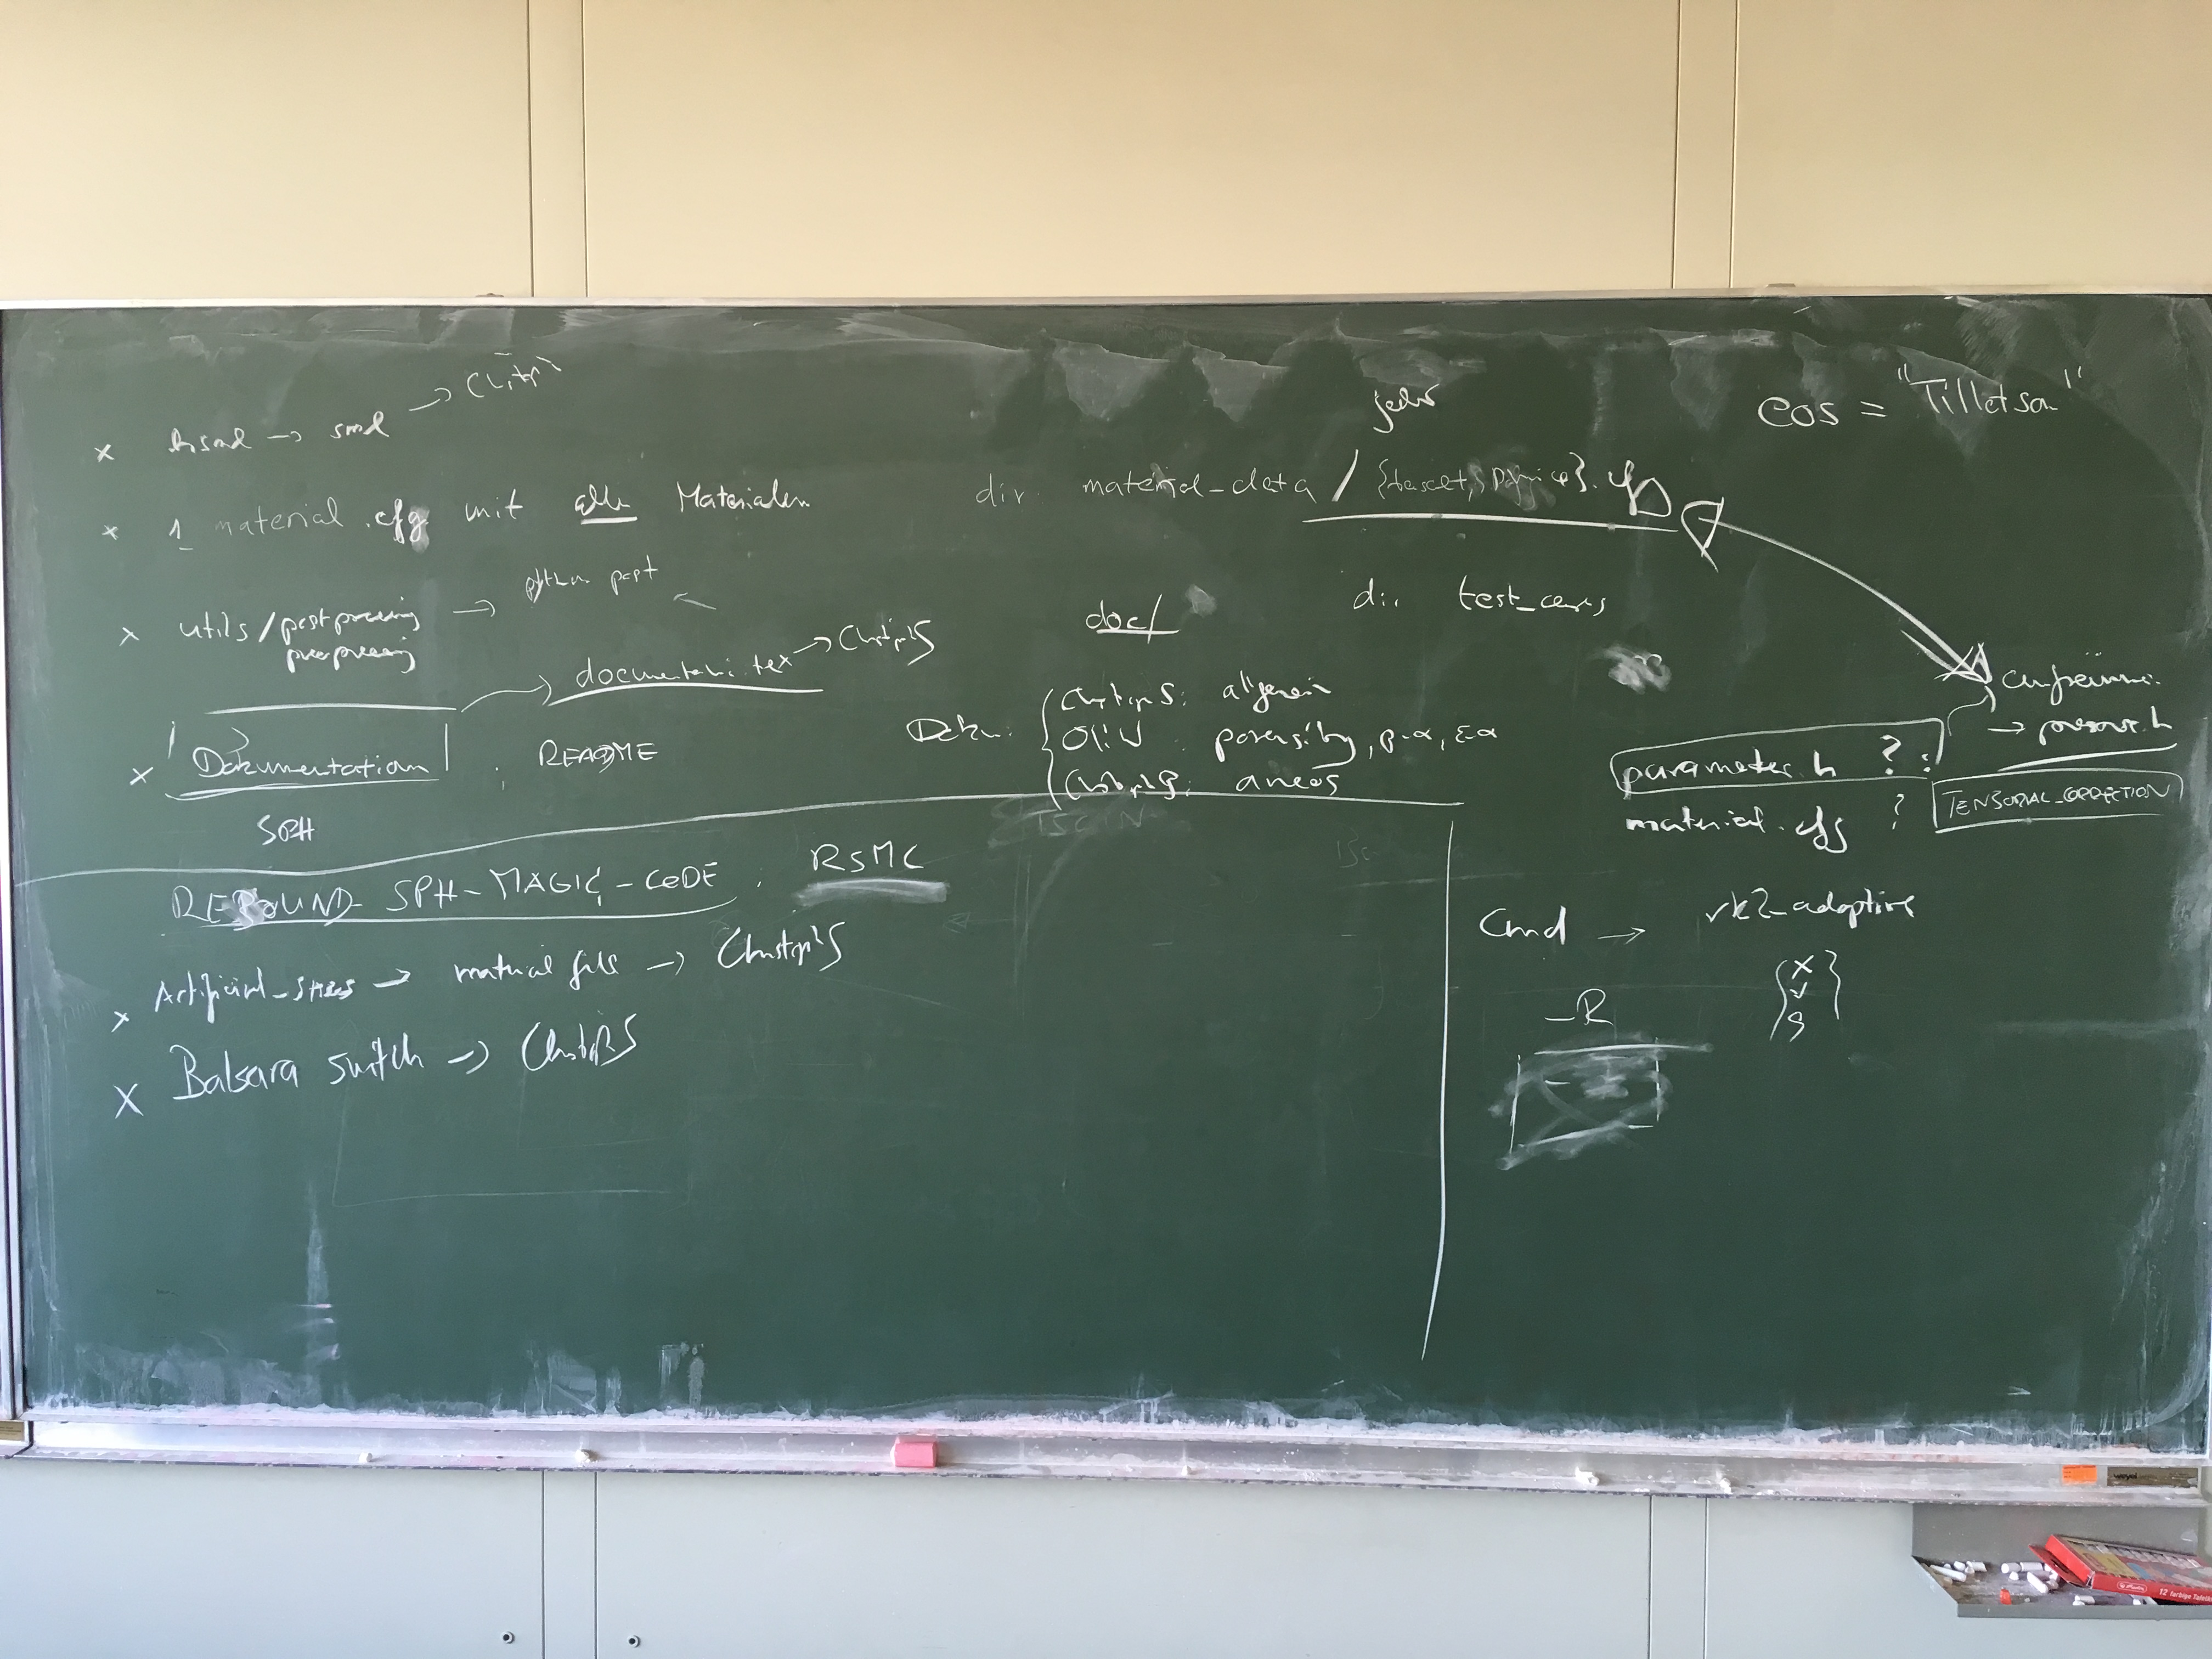
\includegraphics[width=0.5\textwidth]{pic/IMG_1058.jpg}\\
%\crule[unigold]{1em}{1em}~~~\crule[blue]{1em}{1em}~~~\crule[unirot]{1em}{1em}\\
\vfill \normalsize
{\large Version: \today}\\[0.8cm]
written by \\
Christoph Burger, Christoph Schäfer, Oliver Wandel \\ Institut für Astronomie und
Astrophysik \\ Eberhard-Karls-Universität Tübingen}
\date{\vspace{-5ex}}
\pagestyle{fancy}
\fancyhead[RE,RO]{\crule[unigold]{0.7em}{0.5em} ~~~ \nouppercase \leftmark}
\fancyhead[LO]{\crule[unirot]{0.7em}{0.5em}~~~ miluphCUDA}
\fancyhead[LE]{\crule[blue]{0.7em}{0.5em}~~~ miluphCUDA}

\usepackage{xcolor}
\newcommand\crule[3][black]{\textcolor{#1}{\rule{#2}{#3}}}
\definecolor{unirot}{RGB}{165,30,55} %rote Farbe
\definecolor{unigrau}{RGB}{195,195,195} %graue Farbe
\definecolor{unigold}{RGB}{180,160,105} %goldene Farbe
\begin{document}

\sisetup{
    range-units = single
}

% hyperlink colors:
\hypersetup{
    pdftitle={Documentation miluphCUDA},    % title
    pdfauthor={Christoph Schäfer},     % author
    pdfcreator={Christoph Schäfer},   % creator of the document
    colorlinks = {true},
    citecolor = {unirot},
    linkcolor = {unirot},
    %citebordercolor = {red},
    urlcolor = {unirot},
    %linkbordercolor = {red},
    %urlbordercolor = {white}
}
%%%% TITLE PAGE %%%%%%%%%%%%%%%%%%%%%%%%%%%%%%%%%%%%%%%%%%%
\maketitle
\thispagestyle{empty}
\newpage
\tableofcontents
\newpage
\setcounter{page}{1}




\section{Introduction}
\emph{miluphCUDA} was originally the CUDA port of the code \emph{miluph} (see \url{http://www.tat.physik.uni-tuebingen.de/~schaefer/miluph.html}).
It's a Smooth Particle Hydrodynamics (SPH) code for the simulation of fluids as well as solid and porous bodies.
\emph{miluphCUDA} is capable of using various different equation of state (see Sect.~\ref{section:eos}) and the material strength model and a damage model introduced by Benz \& Asphaug for the simulation of brittle solid materials (see Sect.~\ref{section:damage_model}). Self-gravity can be included and is solved using a Barnes-Hut tree (see Sect.~\ref{section:self-gravity}). The code can be used for the simulation of high-velocity impacts and/or self gravitating astrophysical objects or mixed hydro-solid simulations.

The code and its numerics are well described in the publication:

\emph{Schäfer, C.; Riecker, S.; Maindl, T.; Speith, R.; Scherrer, S.; Kley, W.: A Smooth Particle Hydrodynamics Code to Model Collisions Between Solid, Self-Gravitating Objects},

published in Astronomy \& Astrophysics.

Please cite this paper when using our code.


\paragraph*{Copyright and Authors}
Christoph Schäfer and Sven Riecker wrote the basic version of \emph{miluphCUDA}.

Later additions (chronologically):
\begin{itemize}
\item Soil material model: Samuel Scherrer
\item Johnson-Cook material model: Janka Werner
\item Porosity model: Oliver Wandel
\item ANEOS support: Christoph Burger
\item Drucker-Prager and Mohr-Coulomb material model: Christoph Schäfer
\item Navier-Stokes equation: Christoph Schäfer
\end{itemize}

Authors of some additional tools in \verb|test_cases/| or \verb|utils/|:
\begin{itemize}
\item Christoph Burger
\item Thomas I. Maindl
\end{itemize}







\section{Quick Start Guide}
\subsection{Installation steps}
\begin{enumerate}
\item Install CUDA, e.g., from \url{https://developer.nvidia.com/cuda-downloads}
\item Check out \emph{miluphCUDA} from the git repo, e.g.,\\ \verb|git clone git@cpt-milkyway.am10.uni-tuebingen.de:/stoffel/miluphcuda.git|\\
If you do not have an account, email to \emph{ch.schaefer@uni-tuebingen.de} and request one.
\item Install \emph{libconfig}: Download\\
\verb|http://www.hyperrealm.com/libconfig/libconfig-1.4.9.tar.gz|\\
(or a newer version) and
\begin{itemize}
\item \verb|sudo ./configure|
\item \verb|sudo make|
\item \verb|sudo make install|
\end{itemize}
or\\
\verb|apt-get install libconfig9-dev|\\
on Ubuntu/Debian
\item If you want to use HDF5, you need to install \emph{libhdf5} and \emph{libhdf5-dev}
\item Make relevant changes to \emph{parameter.h} to specify all compile-time options
\item Make relevant changes to the \emph{Makefile}: Change the \verb|CUDA_DIR| variable according to your CUDA version. Make sure to use the correct \verb|GPU_ARCH| corresponding to your Nvidia-GPU model. Otherwise the code will \emph{not} work and crash or give wrong results!
Tested CUDA versions with Nvidia-driver versions are given in Tab.~\ref{tab:cuda_driver}.

\begin{table}
\centering
\caption{Tested CUDA versions with Nvidia-driver versions}
\begin{tabular}[h]{p{3cm} p{3cm}}
\hline
CUDA version	&	Nvidia driver	\\
\hline
6.0		&	331.113\\
6.5		&	\\
7.0		&	346.46	\\
7.5		&	352.39, 367.27	\\
8.0		&	375.26, 375.66, 384.111, 390.67	\\
9.0		&	390.67	\\
10.0	&	430.14 \\  \hline
\end{tabular}
\label{tab:cuda_driver}
\end{table}

Unsupported cuda versions so far: $<= 5.0$

Also change the compiler and linker flags in the Makefile according to your system (e.g., \verb|-L| and \verb|-I| for \emph{libhdf5} and \emph{libconfig}).
\end{enumerate}



\subsection{Usage of the code}
The code and its numerics are comprehensively described in the publication:

\emph{Schäfer, C.; Riecker, S.; Maindl, T.; Speith, R.; Scherrer, S.; Kley, W.: A Smooth Particle Hydrodynamics Code to Model Collisions Between Solid, Self-Gravitating Objects},

which is published in Astronomy \& Astrophysics.

Please cite this paper when using our code.


\paragraph*{Compile time options}
The number of threads for some CUDA kernels can be set as compile time options in \emph{timeintegration.h}. You may need to change (if so then probably lower) some values depending on your hardware.

All compile time options related to the physical model have to be set in \emph{parameter.h}!
Please edit and check \emph{parameter.h}. There are comments for each \texttt{\#define}.


\paragraph*{Command line options}
A lot of important settings have to be provided at the command line (see Tab.~\ref{tab:cmd-line-options}, and also \\
\verb|./miluphcuda --help|)

\begin{table}
\centering
\caption{Available command line options.}
\begin{tabular}[b]{p{5cm} p{9cm}}
\hline
Option	&	Purpose		\\
\hline
\verb|-h, --help|			&	print help message	\\
\verb|-G, --information|	&	print information about detected Nvidia GPUs on this host	\\
\verb|-d, --device_id <int>|	&	try to use GPU device with id \verb|<int>| for computation (default: 0)	\\
\verb|-Y, --format|	&	print information about input and output format of the data files	\\
\verb|-v, --verbose|	&	be talkative (stdout)	\\
\verb|-I, --integrator|	&	available Integrators are \verb|euler| (1st order), \verb|euler_pc| and \verb|monaghan_pc| (2nd order), \verb|rk2_adaptive| (2nd order with adaptive time step)	\\
\verb|-Q, --precision|		&	precision of the \verb|rk2_adaptive| integrator (default: 1e-6)	\\
\verb|-n, --num|	&	number of simulation steps	\\
\verb|-H, --hdf5_output|	&	write HDF5 output files (default is no)	\\
\verb|-X, --hdf5_input|   	&	use HDF5 file for input (default is no), file \emph{<string>.XXXX.h5} will be opened (i.e. to open e.g., \emph{impact.0123.h5} pass \verb|impact.0123| to option \verb|-f|)	\\
\verb|-A, --no_ascii_output|	&	disable ASCII output files (not set by default)	\\
\verb|-a, --theta|		&	Theta Criterion for Barnes-Hut Tree (default: 0.5)	\\
\verb|-t, --timeperstep|	&	time for one simulation step (for writing to output files for adaptive integrators)		\\
\verb|-M, --maxtimestep|  &		upper limit for the timestep (\verb|rk2_adaptive|), or timestep size for \verb|euler|, respectively	\\
\verb|-T, --starttime|		&	start time of the simulation	\\
\verb|-f, --filename|		&	name of input data file (default: \emph{disk.0000}); input file name format is something like \emph{<string>.XXXX}, where \emph{XXXX} means runlevel and zeros	\\
\verb|-r, --restart|		&	assume that ASCII input file is old output file	\\
\verb|-m, --materialconfig|		&	name of file containing material parameters for all materials in the simulation		\\
\verb|-k, --kernel|		&	specify the kernel function, available are \verb|wendlandc2|, \verb|wendlandc4|, \verb|wendlandc6|, \verb|cubic_spline|, \verb|quartic_spline|, default: \verb|cubic_spline|		\\
\verb|-s, --selfgravity|	&	include self-gravity		\\
\verb|-D, --directselfgravity| & 	Calculate selfgravity using direct particle-particle force and not the tree (slower) \\
\verb|-L VALUE| &  Check for conservation of angular momentum. (default: off)
    Simulations stops once the relative difference between current angular momentum and initial
    angular momentum is larger than VALUE. \\
\verb|-g, --decouplegravity|	&	decouple hydro time scale from gravitational time scale	\\
\verb|-b, --boundary_ratio|	&	ratio of additional ghost boundary particles (default: 0)	\\
\hline
\end{tabular}
\label{tab:cmd-line-options}
\end{table}

One of the most important switches is \verb|--verbose|, which provides much more helpful output.


\paragraph*{Input file}
In order to run a simulation, you need a simulation input file, that includes at least the coordinates and masses of your initial SPH particle distribution (in case of a HYDRO simulation, for SOLID simulations more columns in the input file are required).
Please use\\
\verb|./miluphcuda --format|\\
to determine the correct input file format, and to display the output file format.


\paragraph*{Material parameter file}
The required material parameters are set in the file \emph{material.cfg}, which is passed via the command line argument \verb|-m|. Refer to the available materials in \verb|material_data/| and the examples in \verb|test_cases/| for the different needed material parameters.


\paragraph*{Usage example}
Example of miluphCUDA invocation (from the colliding rubber rings example in

\verb|test_cases/colliding_rings/|):

\begin{verbatim}
# set the correct LD_LIBRARY_PATH to the cuda libs
export LD_LIBRARY_PATH=/usr/local/cuda-7.5/lib64
# invoke miluphCUDA: use the rk2_adaptive integrator, use HDF5
# output and write 500 output files at simulation times
1.0
2.0
3.0
(...)
500.0
# the files will be named
rings.0001
rings.0002
rings.0003
(...)
rings.0500
# the used miluphCUDA command line is
./miluphcuda -v -I rk2_adaptive -n 500 -H -t 1.0 -f rings.0000 -m material.cfg 
\end{verbatim}



\paragraph*{Porosity usage}
If you want to model one or more materials which are porous, you have to change some things--(*) marked points need to be done for simulations with at least 1 porous material, while (**) marked points need to be done if the regarded material is porous.

In \emph{parameter.h}:
\begin{itemize}
\item (*) you have to switch on \verb|PALPHA_POROSITY|
\end{itemize}

In \emph{material.cfg}:
\begin{itemize}
\item (**) porosity uses \verb|EOS_TYPE_JUTZI| which is \emph{type = 5} for the use of the Tillotson eos (recommended), or \verb|EOS_TYPE_JUTZI_MURNAGHAN| which is \emph{type = 6} for the use of the Murnaghan eos
\item (**) this needs to be added to the eos (it defines the crush-curve and was fitted for porous pumice):
\begin{verbatim}
            porjutzi_p_elastic = 1.0e6;
            porjutzi_p_transition = 6.80e7;
            porjutzi_p_compacted = 2.13e8;
            porjutzi_alpha_0 = 3.0;
            porjutzi_alpha_e = 4.64;
            porjutzi_alpha_t = 1.90;
            porjutzi_n1 = 12.0;
            porjutzi_n2 = 3.0;
\end{verbatim}
The value \verb|porjutzi_alpha_0| needs to be set to the initial distention at the start of the simulation. In this case it is 3.0 which translates to a porosity of Phi = 1 - 1/alpha\_0 = 1 - 1/3.0 = 66.6\%.
\item (**) the value of \verb|till_rho_0| needs to be set to the matrix density of the regarded material
\end{itemize}

In your input file:
\begin{itemize}
\item (*) At the very end of your input file and before you weibull the file the last two variables are \verb|alpha_jutzi| and \verb|p| (the data format can also be checked using the cmd-line option \verb|-Y|, see Tab.~\ref{tab:cmd-line-options}). \verb|alpha_jutzi| is the initial distention at the start of the simulation (the same as in the \emph{material.cfg} file) and \verb|p| needs to be set to 0 so that there isn't any pressure at the start. \verb|p| is needed since dP = P\_new - P\_old is being calculated in the code.
\item (**) The initial density rho (porous density) needs to be set so that rho * alpha\_jutzi = rho\_s (rho\_s is the matrix density which is set in \emph{material.cfg} as till\_rho\_0). This has to match exactly!
\item (**) The mass of the particles also needs to be adjusted to being porous. Normally if you calculate the mass using the density then the mass is already the mass for the porous particle.
\end{itemize}
Please note: for the time beeing, you will also have to set the flag \texttt{flag\_alpha\_quad} in \texttt{pressure.cu} directly
\begin{lstlisting}
int flag_alpha_quad;        /* if this flag is set -> alpha gets calculated by a quadradic equation and not via the crush curve */
\end{lstlisting}


\subsection{A last note}
We do NOT support the use of the code for military purposes.




\section{Code structure}
If you want to add some changes to the code, read and understand \emph{CodingStyle.txt}.

\subsection{Data structure}
We use the struct \verb|Particle| (from \emph{miluph.h}) for storing all information about a SPH particle. The struct depends on the
settings in \emph{parameter.h}.

\subsection{List of files and directory structure}
Table~\ref{tab:file-list} contains a list of the files that are part of the \emph{miluphCUDA} project.

There are additional subdirectories\\
\verb|utils/|\\
\verb|test_cases/|\\
\verb|material_data/|\\
\verb|doc/|\\
that include pre and postprocessing utilities, test-cases, material parameters for \emph{material.cfg}, and this documentation.

\begin{table}
\centering
\caption{List of files in \emph{miluphCUDA}.}
\small
\begin{tabular}[b]{p{6cm} p{9cm}}
\hline
Filename	&	Purpose		\\
\hline
aneos.cu, aneos.h	&	functions for initializing and running ANEOS	\\
artificial\_stress.cu, artificial\_stress.h	&	functions for artificial stress (see Gray, Monaghan, Swift 2001)\\
boundary.cu, boundary.h		&	special treatment of boundaries	\\
checks.h	&	consistency checks of compile time options	\\
cuda\_utils.h	&	CUDA specific functions	\\
damage.cu, damage.h		&	functions for the fragmentation and damage models	\\
density.cu, density.h	&	calculate density or time derivative of density	\\
device\_tools.cu, device\_tools.h		&	\\
euler.cu, euler.h	&	Euler integrator; stress tensor (regolith) and/or deviatoric stress tensor (all other solid materials)	\\
gravity.cu, gravity.h	& functions for the calculation of self gravity \\
internal\_forces.cu, internal\_forces.h	&	compute the change of stress tensor (regolith) and/or deviatoric stress tensor (all other solid materials)	\\
io.cu, io.h		&	functions for input/output, ASCII and HDF5	\\
kernel.cu, kernel.h		&	calculate SPH kernel values	\\
linalg.cu, linalg.h		&	helping functions for matrix operations etcpp.	\\
little\_helpers.cu, little\_helpers.h	&	\\
Makefile	&	Makefile for GNU Make. You'll need to make changes according to your CUDA version and your GPU architecture in this file	\\
material.cfg	&	In this file, you define the material parameters for each materialID that your simulation includes.	\\
memory\_handling.cu, memory\_handling.h	&	functions for memory allocation and copying between host and device	\\
miluph.cu	&	main	\\
miluph.h	&	header file with \verb|Particle| structure definition	\\
parameter.h	&	this file includes all relevant compile time options. You will need to make changes here in order to define your physical model (HYDRO, SOLID, w/o FRAGMENTATION, DIMENSION, ...)	\\
pc\_values.dat	&	mininum absolute values, which are needed for the predictor-corrector integration schemes	\\
plasticity.cu, plasticity.h		&	material models (rheology): Drucker-Prager, Johnson-Cook, von Mises	\\
porosity.cu, porosity.h		&	porosity model following Jutzi et al. (200x)	\\
predictor\_corrector.cu, predictor\_corrector.h	&	Predictor-Corrector integrator with predictor step dt/2, following Monaghan (1983)	\\
predictor\_corrector\_euler.cu, predictor\_corrector\_euler.h		&	Predictor-Corrector integrator with predictor step dt	\\
pressure.cu, pressure.h		&	calculation of the pressure according to the chosen eos; currently there is, for solids: Tillotson eos, Murnaghan eos, Regolith eos (Drucker-Prager model), ANEOS; for porous solids: Jutzi eos (this is Tillotson eos with alpha), Jutzi-Murnaghan eos (this is Murnaghan eos with alpha); for gas: Ideal gas eos, Polytropic gas eos, Isothermal gas eos		\\
rhs.cu, rhs.h	&	right-hand sides	\\
rk2adaptive.cu, rk2adaptive.h	&	RK2 integrator with adaptive time step	\\
soundspeed.cu, soundspeed.h		&	calculation of the soundspeed	\\
stress.cu, stress.h		&	calculation of the stress tensor \\
timeintegration.cu, timeintegration.h	&	calculation of all internal forces of the solid or fluid; calculation of artificial viscosity and artificial stress if defined in \emph{parameter.h}		\\
tree.cu, tree.h		&	calculation of self gravity using a Barnes-Hut Tree (no quadrupoles!)	\\
velocity.cu, velocity.h		&	calculate velocities	\\
viscosity.cu, viscosity.h		&	functions for INVISCID==1. the viscosity ansatz by Cullen \& Dehnen (2010)\\
 & and Navier-Stokes equation \\
xsph.cu, xsph.h		&	functions for the XSPH algorithm	\\
\hline
\end{tabular}
\label{tab:file-list}
\end{table}



\section{Physical model}
In this section, we present the set of partial differential equations from continuum mechanics in Cartesian coordinates
that we apply to model gas and solid bodies.
Throughout this documentation, the Einstein summation rule is used, Greek indices denote spatial coordinates and run from 1 to
3.
\subsection{Mass conservation}
The equation of continuity is the equation of the conservation of mass. It is given in Lagrangian form by
\begin{equation}
\label{eq:conservation_of_mass}
\frac{\mathrm{d} \varrho}{\mathrm{d}t} + \varrho \frac{\partial v^\alpha}{\partial x^\alpha} = 0,
\end{equation}
where $\varrho$ denotes the density and $\vect{v}$ the velocity of the solid body or fluid.
\subsection{Conservation of momentum}
The equation of the conservation of momentum in continuum mechanics for a solid body reads in Lagrangian formulation
\begin{equation}
\label{eq:conservation_of_momentum}
\frac{\mathrm{d} {v^\alpha}}{\mathrm{d}t} =  \frac{1}{\varrho}  \frac{\partial \sigma^{\alpha
\beta} }{\partial x_\beta},
\end{equation}
where $\sigma^{\alpha\beta}$ is the stress tensor given by the pressure $p$ and the deviatoric stress tensor
${S}^{\alpha \beta}$
\begin{equation}
\sigma^{\alpha \beta} = -p \delta^{\alpha \beta} + S^{\alpha \beta},
\end{equation}
with the Kronecker delta $\delta^{\alpha \beta}$.
For a liquid or gas, the deviatoric stress tensor vanishes and the conservation of momentum is given by the Euler
equation
\begin{equation}
\frac{\mathrm{d} {v^\alpha}}{\mathrm{d}t} =  - \frac{1}{\varrho}  \frac{\partial}{\partial x_\beta} p \delta^{\alpha \beta}.
\end{equation}
\subsection{Conservation of internal energy}
The equation of the conservation of the specific internal energy $u$ for an elastic body is given in Lagrangian formulation by
\begin{equation}
\label{eq:conservation_internal_energy}
\frac{\mathrm{d} u }{\mathrm{d} t} = - \frac{p}{\varrho} \frac{\partial v ^\alpha}{\partial x^\alpha} + \frac{1}{\varrho}
S^{\alpha \beta} \dot{\varepsilon}^{\alpha \beta},
\end{equation}
with the strain rate tensor $\dot{\varepsilon}^{\alpha \beta}$ given by eq.~(\ref{eq:strain_rate_tensor}).
\subsection{Constitutive equations}
In contrast to fluid dynamics, the set
(\ref{eq:conservation_of_mass};\ref{eq:conservation_of_momentum};\ref{eq:conservation_internal_energy}) of partial
differential equations is not sufficient to describe the dynamics of an elastic solid body, since the time evolution of
the deviatoric stress tensor $S^{\alpha \beta}$ is not yet specified. For the elastic behavior of a solid body, the
constitutive equation is based on Hooke's law. Extended to three dimensional deformations, it reads
%
\begin{equation}
S^{\alpha \beta} \sim 2 \mu \left( \varepsilon^{\alpha \beta} - \frac{1}{3} \delta^{\alpha \beta} \varepsilon^{\gamma
\gamma} \right).
\end{equation}
%
Here, $\mu$ denotes the material dependent shear modulus and $\epsilon^{\alpha \beta}$ is the strain tensor.
%
For the time evolution, it follows (for small deformations)
%
\begin{align}
\label{eq:stresstensor_evolution}
\frac{\mathrm{d}}{\mathrm{d}t}S^{\alpha \beta} =  2\mu \left( \dot{\varepsilon}^{\alpha \beta} - \frac{1}{3}
\delta^{\alpha \beta} \dot{\varepsilon}^{\gamma \gamma} \right)   &  \\  & +  \mathrm{rotation~terms,} \nonumber
\end{align}
%
%
where $\dot{\varepsilon}^{\alpha \beta}$ denotes the strain rate tensor, given by
\begin{equation}
\label{eq:strain_rate_tensor}
\dot{\varepsilon}^{\alpha \beta} = \frac{1}{2} \left( \frac{\partial v^\alpha}{\partial x^\beta} + \frac{\partial
v^\beta}{\partial x^\alpha} \right).
\end{equation}
%
The rotation terms in eq.~(\ref{eq:stresstensor_evolution}) are needed since the constitutive equations have to be
independent from the material frame of reference. There are various possibilities to achieve this. The usual approach
for particle codes is the Jaumann rate form. The rotation terms
of the Jaumann rate form are
%
\begin{equation}
\label{eq:rotation_terms}
S^{\alpha \gamma} R^{\gamma \beta} - R^{\alpha \gamma} S^{\gamma \beta},
\end{equation}
%
with the rotation rate tensor
%
\begin{equation}
R^{\alpha \beta} = \frac{1}{2} \left( \frac{\partial v^\alpha}{\partial x^\beta} - \frac{\partial v^\beta}{\partial x^\alpha}
\right).
\end{equation}
%
Together, eqs.~(\ref{eq:stresstensor_evolution}) and (\ref{eq:rotation_terms}) determine the change of deviatoric
stress due to deformation of the solid body.
%
\subsection{Equation of state}
\label{section:eos}
The equation of state relates the thermodynamic variables density $\varrho$, pressure $p$, and specific internal energy
$u$. We provide a short description about the equation of states that are implemented in the code.
%
\subsubsection{Liquid equation of state}
For small compressions and expansions of a liquid, the pressure depends linearly on the change of density.
Assume $\varrho_0$ is the initial density of the uncompressed liquid. Then, the liquid equation of state reads
%
\begin{equation}
p = c_\mathrm{s}^2 ( \varrho - \varrho_0 ).
\end{equation}
%
Here, $c_\mathrm{s}$ denotes the bulk sound speed of the liquid, which is related to the bulk modulus $K_0$ and the initial
density by
%
\begin{equation}
c_\mathrm{s}^2 = \frac{K_0}{\varrho_0}.
\end{equation}
%
If the density $\varrho$ falls strongly beyond the value of the initial density $\varrho_0$, the liquid equation of
state fails because the liquid forms droplets and attracting forces vanish. To account for this
behavior, the pressure is set to zero as
soon as the ratio $\varrho/ \varrho_0$ drops below $0.8-0.95$ \citep{melosh1996impact}.
%
\subsubsection{Murnaghan equation of state}
The Murnaghan equation of state is an extension of the liquid equation of state (see, e.g.,\ \citealt{melosh1996impact}). In contrast to the liquid equation of
state, the pressure now depends nonlinearly on the density
%
\begin{equation}
p = \frac{K_0}{n_M} \left[ \left( \frac{\varrho}{\varrho_0}\right)^{n_M} -1  \right],
\end{equation}
%
with the zero pressure bulk modulus $K_0$ and the constant $n_M$. The Murnaghan equation of state is limited to
isothermal compression. Parameters for various materials can be found in the literature, e.g.,\ \cite{melosh1996impact}.
%
%
\subsubsection{Tillotson equation of state}
\label{section:tillotson}
The Tillotson equation of state was originally derived for high-velocity impact simulations \citep{til62}.
There are two domains depending upon the material specific energy density $u$. In the case of compressed regions ($\varrho \geq
\varrho_0$) and $u$ lower than the energy of incipient vaporization $E_\mathrm{iv}$ the equation of state reads
%
\begin{align}\label{eq:tillo1}
p = \left[ a_T + \frac{b_T}{1+u/(E_0 \eta^2)} \right]\varrho u + A_T\chi + B_T\chi^2,
\end{align}
%
with $\eta = \varrho / \varrho_0$ and $\chi = \eta-1$.
In case of expanded material ($u$ greater than the energy of complete vaporization $E_\mathrm{cv}$) the
equation of state takes the form
%
\begin{align}\label{eq:tillo2}
p = & a_T\varrho u +  \left[ \frac{b_T\varrho u}{1+u/(E_0 \eta^2)} \right. \nonumber \\
 & \; + \left. A_T\chi \exp \left\{-\beta_T \left(\frac{\varrho_0}{\varrho}-1\right)\right\} \right] \nonumber \\ & \qquad \qquad
 \times  \exp
 \left\{-\alpha_T\left(\frac{\varrho_0}{\varrho}-1\right)^2\right\}.
\end{align}
%
The symbols $\varrho_0$, $A_T$, $B_T$, $E_0$, $a_T$, $b_T$, $\alpha_T$, and $\beta_T$ are material dependent
parameters.

In the partial vaporization $E_\mathrm{iv} < u < E_\mathrm{cv}$, $p$ is linearly interpolated between the pressures
obtained via (\ref{eq:tillo1}) and (\ref{eq:tillo2}), respectively. For a more detailed description see
\cite{melosh1996impact}.

The Tillotson equation of state has the advantage of being computational very simple, while sophisticated enough for the
application over a wide regime of physical conditions, such as high-velocity collisions and impact cratering.

\subsubsection{ANEOS}
If you want to use the tabulated ANEOS eos for some material you need three things:
\begin{enumerate}
\item A file containing the ANEOS lookup-table data. These files can be generated externally with the aid of the external project \emph{miluphANEOS}, a Fortran code that calls ANEOS subroutines directly. See there for further instructions.
\item Suitable entries in \emph{material.cfg} for that material. See the available materials in \verb|material_data/|.
\item Consistent initial conditions. For setting up homogeneous bodies you can use \verb|aneos_rho_0| and \verb|aneos_e_norm| initially (see \emph{material.cfg}). This, and also the direct generation of equilibrated (large) bodies, can be done by the initial conditions code in the external project \emph{Relaxation}.
\end{enumerate}
\subsubsection{Locally-isothermal gas}
\texttt{EOS\_TYPE\_LOCALLY\_ISOTHERMAL\_GAS}
\begin{align}
    p & = c_s^2 \varrho
\end{align}
\subsubsection{Perfect gas equation}
\texttt{EOS\_TYPE\_IDEAL\_GAS}
\begin{align}
    p & = (\gamma-1) \varrho e
\end{align}
\subsubsection{Polytropic Gas}
\texttt{EOS\_TYPE\_POLYTROPIC\_GAS}
\begin{align}
    p & = K \varrho^\gamma
\end{align}
\subsection{Plastic material equations}
Together with the equation of state, the set of equations
(\ref{eq:conservation_of_mass};\ref{eq:conservation_of_momentum};\ref{eq:conservation_internal_energy}) can be used to
describe the dynamics of a solid body in the elastic regime. We apply the von Mises yield
criterion \citep{vonmises1913} to model plasticity. The deviatoric stress is
limited by
%
\begin{equation}
S^{\alpha \beta} \rightarrow f_Y S^{\alpha \beta},
\end{equation}
where the factor $f_Y$ is computed from
\begin{equation}
f_Y = \mathrm{min} \left[ Y_0^2/3J_2, 1 \right],
\end{equation}
with the second invariant of the deviatoric stress tensor $J_2$ given by
%
\begin{equation}
J_2 = \frac{1}{2} S^{\alpha \beta} S_{\alpha \beta},
\end{equation}
and the material dependent yield stress is $Y_0$.
%
\subsection{Damage model for brittle material}
\label{section:damage_model}
Since one major application of the newly developed code includes the simulation of the collision between
brittle planetesimals, we included a fragmentation model. Physically, fracture is related to the
failure of atomic or molecular bonds. If an applied force on a solid brittle body is large enough to break the atomic
bonds, the material begins to fracture and develop cracks. A successful continuum model for fragmentation was
derived by \cite{grady:1980} and first implemented in a SPH code by \cite{benz:1995}. The model is based on
two assumptions: brittle materials contain so-called flaws that are sources of weakness leading to activation and
growth under tensile loading, and dynamic fracture depends on the rate of tensile loading. In other words, material that
is slowly pulled apart develops fewer cracks than material that experiences higher strain rates, since one single
crack cannot relieve the higher tensile stress, and hence more flaws get activated leading to more cracks and
consequently more damage.

The scalar parameter damage $d$ parametrizes the influence of cracks on a given volume
\begin{equation}
0 \leq d \leq 1,
\end{equation}
and is defined in a way that $d=0$ represents an undamaged, intact material and $d=1$ a fully damaged material that
cannot undergo any tension or deviatoric stress. In this manner, a material with $d=0.5$ experiences half the stress and
tension of undamaged material with $d=0$.


Damage reduces the strength under tensile loading and the elastic stress $\sigma^{\alpha \beta}$ is decreased
by the factor $(1-d)$, or in more detail
%
\begin{equation}
\sigma^{\alpha \beta}_d = -\hat{p} \delta^{\alpha \beta} + (1-d) S^{\alpha \beta},
\end{equation}
with
\begin{equation}
\hat{p} = \left\{ \begin{array}{ll} p &  \mathrm{for} \ p \geq 0 \\
  (1-d) p &   \mathrm{for} \ p < 0 \end{array} \right. .
\end{equation}
%
The number of flaws per unit volume in a brittle body with failure strains that are lower than $\varepsilon$, is given by
the Weibull distribution \citep{weibull:1939}
%
\begin{equation}
n(\varepsilon) = k \varepsilon^m,
\end{equation}
with the two Weibull parameters $k$ and $m$. Typical values for basalt are $m=16$, $k=\SI{1e61}{\per
\cubic\metre}$ \citep{2007JGRE..112.2001N}.

As soon as a spherical volume $V= \nicefrac{4}{3} \, \pi R_s^3$ undergoes a strain greater than its lowest activation threshold
strain, damage starts to grow according to
%
\begin{equation}
\label{eq:damage_growth}
\frac{\mathrm{d}}{\mathrm{d}t} d^{\nicefrac{1}{3}} = \frac{c_\mathrm{g}}{R_s},
\end{equation}
%
with the constant crack growth velocity $c_\mathrm{g}$. The crack growth velocity is chosen to be 40\% of the velocity of
a longitudinal elastic wave in the damaged material
%
\begin{equation}
c_\mathrm{g} = \num{0.4} \frac{1}{\varrho} \sqrt{ K_0 + \nicefrac{4}{3} (1-d) \mu}.
\end{equation}
%
The fracture model requires the distribution of activation threshold strains (flaws) among the brittle body's SPH particles as a preprocessing step to the simulations.
%

We apply the algorithm introduced by \cite{benz:1995} with the following approach: Flaws
are distributed randomly among the brittle particles until each particle has been assigned with at least one activation
threshold. We let $N_\mathrm{flaw}$ be the number of totally distributed activation flaws. For each flaw $j$, $1\leq j \leq
N_\mathrm{flaw}$, a particle $a$ is chosen randomly and assigned with the activation threshold strain derived from the
Weibull distribution $\varepsilon_{a,j}$,
%
\begin{equation}
\varepsilon_{a,j} = \left[ \frac{j}{kV} \right]^{\nicefrac{1}{m}},
\end{equation}
%
where $V$ is the volume of the brittle material and $k$ and $m$ are the material dependent Weibull parameters. Using
this procedure, each particle gets at least one flaw and on average a total of $N_\mathrm{flaws} = N_p \ln N_p$ flaws
are distributed. This number of flaws has to be stored in the memory during the simulation and is the
main memory consumer in simulations with brittle materials.


During the simulation, once a particle undergoes a strain greater than its lowest activation threshold strain, damage
grows according to a modified version of eq.~(\ref{eq:damage_growth})
%
\begin{equation}
\frac{\mathrm{d}}{\mathrm{d} t} d^{\nicefrac{1}{3}} = n_\mathrm{act} \frac{c_\mathrm{g}}{R_s},
\end{equation}
%
where $n_\mathrm{act}$ is the number of activated flaws of the particle. This modification accounts for the accumulation
of cracks.

Additionally, a damage limiter is included in the model. Since a particle has in general more than only one activation
threshold, its behavior under tensile loading would be given by the flaw with the lowest activation threshold.  To
prevent this, the damage of the particle is limited by the ratio between the number of activated flaws $n_\mathrm{act}$
and the number of total flaws $n_\mathrm{tot}$ of this particle
%
\begin{equation}
d_\mathrm{max} = \frac{n_\mathrm{act}}{n_\mathrm{tot}}.
\end{equation}
%
In other words, a particle can only be totally damaged if all of its flaws are activated.

In order to determine if a particle exceeds one of its threshold strains during the simulation, we need to derive the
local scalar strain from the three-dimensional stress. \cite{benz:1995} suggest computing the local scalar strain
$\varepsilon$ from the maximum tensile stress $\sigma_\mathrm{max} = \max [\sigma_1, \sigma_2, \sigma_3 ]$, where
$\sigma_\gamma$ are the principal stresses determined by a principal axis transformation of the stress tensor
$\sigma^{\alpha \beta}$, which is already reduced by damage and yield strength
%
\begin{equation}
\varepsilon = \frac{\sigma_\mathrm{max}}{(1-d) E}.
\end{equation}
The Young's modulus $E$ of the intact material given by the bulk and shear moduli is written as
\begin{equation}
E = \frac{9 K \mu}{3K+\mu}.
\end{equation}
%
%
\section{Self-gravity with Barnes-Hut Tree}
\label{section:self-gravity}
%
We have implemented the efficient routines for Barnes-Hut tree builds and calculation of the gravitational forces for GPUs introduced by \cite{burtscher:2011}. The algorithm
for the tree generation is explained at the end of this section.

\cite{1986Natur.324..446B} were the first to use a hierarchical tree to calculate the gravitational forces between N
bodies. Their approximation algorithm uses a tree-structured hierarchical subdivision of space into cubic cells, each of
which is divided into $2^D$ subcells. The algorithm has the order ${\cal O}(N \log N)$ compared to the ${\cal O}(N^2)$
algorithm of the direct sum. The basic idea is that only nearby particles have to be treated individually during the
calculation of the gravitational force on a specific particle. Distant nodes of the tree can be seen as one single
particle sitting at the center of mass of the specific tree node and carrying the mass of all the particles that reside
in this node. Although different algorithms for the computation of self-gravitational forces exist, the hierarchical
tree method is specially suited for the use in combination with SPH. As a side product of the computation of the
gravitational forces, the hierarchical tree is constructed for each individual time step and hence, a geometrical hierarchy
of the SPH particles (leaves of the tree) is available at all time of the computation. It can be used to determine the
interaction partners for the SPH algorithm by performing a tree walk for each individual particle \citep{hernquist:1989}. Although the tree
walks may take longer than the search through a helping grid, the interaction partner search may be faster because, in
any case the tree build needs to be carried out in simulations with self-gravity.

We calculate the center of mass and total mass of every node in the tree to calculate the gravitational force exerted on the SPH particles. We call these objects pseudo-particles in the following. Now, for each SPH
particle, we perform a tree walk over all nodes.
With the use of the
$\vartheta$ criterion, we identify whether a pseudo-particle sitting in the node may be used for the calculation of the
gravitational force acting on our particle or whether we have to descend further down in the tree. The $\vartheta$ criterion is given by
%
\begin{equation}
\frac{s_{d_t}}{r_{pp}} < \vartheta,
\end{equation}
%
where $s_{d_t}$ denotes the edge length of the tree node containing the pseudo-particle and $r_{pp}$ is the distance
between the SPH particle and the pseudo-particle.
The gravitational force from the pseudo-particle acting on the particle $a$ is then given by
%
\begin{equation}
\label{eq:gravitational_force}
\vect{F_a} = \frac{Gm_a m_p}{r_{pp}^3} \left( \vect{x_a} - \vect{x_p} \right),
\end{equation}
where $\vect{x_p}$ and $m_p$ denote the location and the mass of the pseudo-particle, respectively.
To avoid numerical instabilities, the distance between the pseudo-particle and the particle is smoothed.

\cite{1989ApJS...70..389B} present a detailed error analysis for their tree algorithm. They find consistent accuracies
of the algorithm for $\vartheta=0.3$  with the consideration of the monopoles of the tree compared to $\vartheta=0.7$
and the additional calculation of the quadrupoles for each tree node. The error scales with $\vartheta^2$ and $\sqrt{N_p}$. For the sake of memory saving, we calculate only the monopoles of the tree and use
$\vartheta \leq 0.5$ in our simulations including self-gravity instead of the usual value of $0.8$.
%


We have implemented the Barnes-Hut tree strictly following the efficient implementation for N-body calculations with
CUDA by \cite{burtscher:2011}. The hierarchical decomposition is recorded in an octree. Since CUDA does not allow the
use of pointers, which is convenient for the handling of trees, e.g.,\ allows for recursive programming of tree walks, we
use one large index array for all SPH particles and all tree nodes, which we call {\tt childList}. This memory is
allocated dynamically at the start of the simulation run. The maximum
number of tree nodes is given by $\mathrm{ceil}[2.5 \times N_p]$, where $N_p$ is the number of SPH particles in the
simulation. For each tree node there are $N_\mathrm{children}$ entries in {\tt childList}, where $N_\mathrm{children}$
is simply given by the dimension
\begin{equation}
N_\mathrm{children} = 2^D.
\end{equation}
The tree is constructed in a way that the $N_p$ particles reside in $N_p$ leaves in the end.
At first, the root of the tree is constructed from the geometry of the particle distribution. The computational domain
(in three dimensions) is given by the cube, which encloses all SPH particles. This cube has the edge length
\begin{equation}
s_0 = \max_{\alpha \in D}  \left[ \max_{a,b \in N_p} \left[ x_a^\alpha - x_b^\alpha \right] \right]
\end{equation}
and defines the edge length of the root node.
The edge length of a tree node of depth $d_t$ is given by
\begin{equation}
s_{d_t} = \left[ \frac{1}{2}\right]^{d_t} s_0.
\end{equation}
Starting from the root node, the particles are inserted into the tree in the following way. In the beginning, all but
one (the root node) entry in {\tt childList} are $-1$, corresponding to the status "no kid".  All particles are
distributed among the threads on the GPU.  Now $N_\mathrm{threads}$ threads on the GPU start to compare the locations of their
SPH particles with the position of the root node to determine the childindex. Since there are many more threads than
children (especially in the beginning of the algorithm), we need to avoid race conditions actively. To accomplish this, we add the
status $-2$ or "locked" to the {\tt childList} and use the CUDA\-function "atomic compare and save" {\tt atomicCAS} to
lock an entry in the {\tt childList}. This functions checks first if the specific index is already locked. If the index
in {\tt childList} is already locked, the thread waits for the other threads to finish and restarts its attempt. If the
index is not locked, the threads read the index value, which may be $-1$ in the beginning or a different node index,
and saves it. Now, the second round starts and the children of the root node are already filled with SPH particles that
were sorted there. Since leaves or particles cannot have children by definition, new inner tree nodes have to be
generated. A new inner tree node has half of the edge length from its parent. New inner tree nodes are added until both
particles, the new particle and the particle in the parent node, can be sorted into two different leaves. As soon as
both particles reside in different leaves, the thread writes and cancels the lock.

When we want to calculate the gravitational forces between the SPH particles, we have to calculate the positions
and locations of the pseudo-particles in the tree. We use the algorithm presented by \cite{burtscher:2011} in the
following manner to determine the pseudo-particle in a specific node: For each inner node, we start in parallel for
$N_\mathrm{threads}$ a CUDA kernel that picks the last $N_\mathrm{threads}$ added inner nodes, for which we
calculate the center of mass and total mass at first. If the inner nodes are not leaves, the thread looking at these
nodes and has to wait for all other threads to end beforce continuing because it needs the location and mass of the
pseudo-particles in these nodes. This is again done by the use of $-1$ as the initial mass of a pseudo-particle. When the
thread finishes the calculation for its node, it moves up one tree depth and continues with the next node. The
implementation of Burtscher is especially designed for CUDA, regarding memory access and parallelization.
%
%


\section{SPH representation of the equations}
\subsection{Settings in \texttt{parameter.h}}
The code allows to choose between two different SPH representations of the conservation of momentum
and internal energy equation. In the following for \texttt{SOLID==1}.
\subsubsection{\texttt{SPHEQUATIONS == SPH\_VERSION1}}
The acceleration for particle $a$ is given by
\begin{align}
    \frac{\mathrm{d} v^\alpha_a}{\mathrm{d} t} = \sum_b m_b \left( \frac{\sigma^{\alpha
    \beta}_a}{\varrho_a^2} + \frac{\sigma^{\alpha \beta}_b}{\varrho_b^2} \right ) \frac{\partial
    W_{ab}}{\partial x_a^\beta}.
\end{align}
\subsubsection{\texttt{SPHEQUATIONS == SPH\_VERSION2}}
The acceleration for particle $a$ is given by
\begin{align}
    \frac{\mathrm{d} v^\alpha_a}{\mathrm{d} t} = \sum_b m_b \left( \frac{\sigma^{\alpha
    \beta}_a + \sigma^{\alpha \beta}_b}{\varrho_a  \varrho_b} \right ) \frac{\partial
    W_{ab}}{\partial x_a^\beta}.
\end{align}

\section{Kernel Function}
Several kernel functions are available via command line parameter \texttt{-k/-{}-kernel}. Information about
which kernel is implemented is provided by the standard \texttt{miluphCUDA} help option \texttt{-h/-{}-help}.
In the following sections, $h$ denotes the smoothing length, $q$ is the ratio between distance and
smoothing length, $q=\frac{x_{ab}}{h}$, where $x_{ab}=\left|{\mathbf{x}_a -
\mathbf{x}_b}\right|$ is the distance between particle $a$ and $b$. Please note, that in contrast to
the original definition of the smoothing length, the interaction radius in \texttt{miluphCUDA} is
given by $h$, not $2h$.

\subsection{variable and fixed smoothing length}
The code supports variable and fixed smoothing lengths. Please set \texttt{VARIABLE\_SML} to $1$ in \texttt{parameter.h}
if you want a variable smoothing length. You can additionally choose between a fixed number of interaction partners by setting
\texttt{FIXED\_NOI} to $1$ or the code integrates the time evolution of the smoothing length via
\begin{equation}
    \frac{\mathrm{d} h}{\mathrm{d}t} = \frac{h}{d} \nabla \cdot \vec{v},
\end{equation}
where $d$ denotes the dimension if you set \texttt{INTEGRATE\_SML}. Additionally, please set two factors for the minium and maximum allowed smoothing length
in \texttt{material.cfg}, namely \texttt{factor\_sml\_min} and \texttt{factor\_sml\_max}. The minimum  (maximum) allowed
smoothing length is then given by \texttt{factor\_sml\_min * sml} (\texttt{factor\_sml\_max * sml}).
\subsection{spline kernels}
\subsubsection{cubic spline}
Standard cubic spline kernel by \cite{1985A&A...149..135M}, chosen by command line option \texttt{-k
cubic\_spline}.
\begin{align}
    W(q) = \frac{\sigma}{h^d} \left\{
    \begin{array}{ll}
        ( 6 q^3 - 6q^2  + 1 ) & \quad \mbox{for} \quad 0 \leq q < \frac{1}{2} \\
        2(1 - q)^3 & \quad \mbox{for} \quad \frac{1}{2} \leq q \leq 1 \\
        0 & \quad \mbox{for} \quad q > 1.
    \end{array}
    \right.
\end{align}
where $d$ denotes the dimension, and $\sigma$ is the normalization constant $\frac{4}{3}$,
$\frac{40}{7\pi}$ and $\frac{8}{\pi}$ for 1D, 2D, and 3D, respectively.
\subsubsection{quartic spline}
Quartic spline kernel \citep{2012MNRAS.425.1068D}, chosen by command line option \texttt{-k
quartic\_spline}.
\begin{align}
    W(q) = \frac{\sigma}{h^d} \left( \left(1-q\right)_+^4 -5\left(\frac{3}{5}-q\right)_+^4 +
    10\left(\frac{1}{5}-q\right)_+^4\right) \qquad \mbox{for} \quad 0 \leq q < 1
\end{align}
where $d$ denotes the dimension, and $\sigma$ is the normalization constant $\frac{5^5}{768}$,
$\frac{3\cdot5^6}{2398\pi}$ and $\frac{5^6}{512\pi}$ for 1D, 2D, and 3D, respectively.


\subsection{Wendland kernels}
\subsubsection{Wendland C2}
Wendland C2 kernel \citep{2012MNRAS.425.1068D}, chosen by command line option \texttt{-k
wendlandc2}.
\begin{align}
    W(q) = \frac{\sigma}{h^d} \left\{
    \begin{array}{ll}
        (1-q)_+^4 (1+4q) & \quad \mbox{for 2D and 3D and} \quad 0 \leq  q < 1 \\
        (1-q)_+^3 (1+3q) & \quad \mbox{for 1D and} \quad 0 \leq  q < 1 \\
        0 & \quad \mbox{for} \quad q >= 1.
    \end{array}
    \right.
\end{align}
where $d$ denotes the dimension, and $\sigma$ is the normalization constant $\frac{5}{4}$,
$\frac{7}{\pi}$ and $\frac{21}{2\pi}$ for 1D, 2D, and 3D, respectively\footnote{$(\cdot)_+ \equiv
\max\{0,\cdot\}$}.
\subsubsection{Wendland C4}
Wendland C4 kernel \citep{2012MNRAS.425.1068D}, chosen by command line option \texttt{-k
wendlandc4}.
\begin{align}
    W(q) = \frac{\sigma}{h^d} \left\{
    \begin{array}{ll}
        (1-q)_+^6 (1+6q+\frac{35}{3}q^2) & \quad \mbox{for 2D and 3D and} \quad 0 \leq  q < 1 \\
        (1-q)_+^5 (1+5q+8q^2) & \quad \mbox{for 1D and} \quad 0 \leq  q < 1 \\
        0 & \quad \mbox{for} \quad q >= 1.
    \end{array}
    \right.
\end{align}
where $d$ denotes the dimension, and $\sigma$ is the normalization constant $\frac{3}{2}$,
$\frac{9}{\pi}$ and $\frac{495}{32\pi}$ for 1D, 2D, and 3D, respectively.
\subsubsection{Wendland C6}
Wendland C6 kernel \citep{2012MNRAS.425.1068D}, chosen by command line option \texttt{-k
wendlandc6}.
\begin{align}
    W(q) = \frac{\sigma}{h^d} \left\{
    \begin{array}{ll}
        (1-q)_+^8 (1+8q+25q^2+32q^3) & \quad \mbox{for 2D and 3D and} \quad 0 \leq  q < 1 \\
        (1-q)_+^7 (1+7q+19q^2+21q^3) & \quad \mbox{for 1D and} \quad 0 \leq  q < 1 \\
        0 & \quad \mbox{for} \quad q >= 1.
    \end{array}
    \right.
\end{align}
where $d$ denotes the dimension, and $\sigma$ is the normalization constant $\frac{55}{32}$,
$\frac{78}{7\pi}$ and $\frac{1365}{64\pi}$ for 1D, 2D, and 3D, respectively.

\subsection{spiky kernels}
\subsubsection{Desbrun \& Cani spiky kernel}
\begin{align}
    W(q) = \frac{\sigma}{h^d} \left\{
    \begin{array}{ll}
        (1-q)^3  & \quad \mbox{for} \quad 0 \leq  q < 1 \\
        0 & \quad \mbox{for} \quad q >= 1.
    \end{array}
    \right.
\end{align}
where $d$ denotes the dimension, and $\sigma$ is the normalization constant
$\frac{10}{\pi}$ and $\frac{15}{\pi}$ for 2D and 3D, respectively.

\bibliographystyle{abbrvnat}
\bibliography{miluphcuda_documentation}
\end{document}
